\documentclass[main.tex]{subfiles}
\begin{document}

\chapter{Program Logic} 
	\section{Overview}
	This project used the AVR version of the C programming language (ANSI C with
	binary number support). The AVR development suite (avr-dude, avr-gcc, etc) was
	used to compile and download the program to the microcontroller. 
	
	The Atmega328p application program uses two interrupts to control the external
	display and temperature conversion tasks of the program asynchronously. An
	eight bit timer and ten bit analog to digital converter are used to control
	the execution of the above interrupts. 
	
	\figref{progLogic} shows a flow diagram of the program logic. The Atmega328p
	ADC and Timer control the execution of their respective interrupt service
	routines (or ISR). The ADC ISR handles the conversion of ADC conversion values
	(ADC values) to temperature via \lstinline{setTemp()} which intern displays
	the result via \lstinline{setNum()}. The Timer ISR handles setting the seven
	segment display output.
	
	\begin{figure}[H]
		\begin{center}
			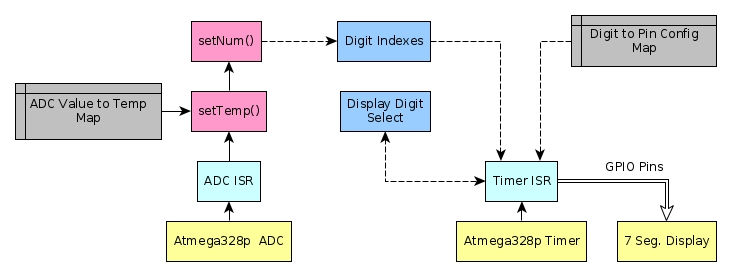
\includegraphics[width=\linewidth]{ProgramLogic.jpg}
		\end{center}
		\caption{Thermometer Program Logic}
		\label{fig:progLogic}
	\end{figure}

	\section{ADC and Timer Overview}
	The Atmega328p has a ten bit successive approximation analog to digital
	converter (noted as ADC). Successive approximation is an analog to digital
	conversion method in which the input signal is constantly compared to the
	output of a guessed analog value (which is stored digitally in an n-bit
	register and is then converted to an analog signal using a digital to analog
	converter). After all n bits of the converter are set the ADC raises a
	conversion completion interrupt flag. It is then that the ADC Interrupt
	Service Routine (or ADC ISR) is called to handle temperature conversion (see
	the ADC to Temperature Conversion section below). See \figref{adcSA} for the
	basics of successive approximation.

		\begin{figure}[H]
			\begin{center}
				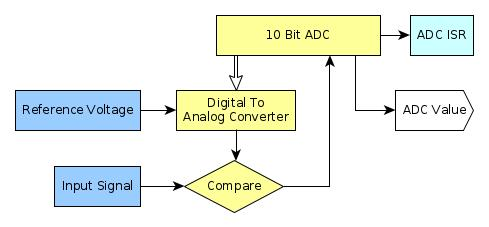
\includegraphics[width=\linewidth]{adc.jpg}
			\end{center}
			\caption{ADC Successive Approximation}
			\label{fig:adcSA}
		\end{figure}
	
	An eight bit timer is used to handle the temperature display. The timer was
	configured to run at approximately fifty-two kilohertz in Clear Timer on
	Compare mode. CTC mode is an operation mode of the timer in which the internal
	counter is reset when the counter matches the value stored in the timer's
	output compare register. Once the timer is reset a timer interrupt vector flag
	is set and the timer ISR is called to handle the display (see the Two Digit
	display section below).

	\section{Two Digit Display}
		\subsection{Single Digit Display Control}
		The two digit seven segment display is controlled by the Atmega328p via two GPIO
		ports. PORTD controls the digit to display and PORTC controls the digit
		selection. An array maps the digits 0 through 9 to their respective pin
		configuration. A given digit is displayed by setting PORTD to the respective
		value in the digit mapping array. For example, if 3 were the digit to display
		then PORTD is set to the value stored in the mapping array at index 3. 

		\subsection{Two Digit Display Multiplexing}
		To display a two digit number a multiplexing method is used. PORTC on the
		Atmega328p is used to control which digit on the seven segment display is
		activated. When the digits are alternatively toggled at a frequency larger
		than 10kHz they appear as if they are displaying simultaneously. The timer  
		ISR handles the toggling of the displays of the two digits.

		\subsection{Display Digit Interface}
		The two digit number to display is stored as two variables which
		contain the indexes to the mapping array; one index per digit. The value to
		display can then be set by calling \lstinline{setNum()} which handles
		storing a two digit number in the index variables. This function can be
		called at any point in the program to set the display.

	\section{ADC to Temperature Conversion}
		\subsection{Obtaining the ADC Conversion Result (or ADC value)}
		The ADC uses two eight bit registers to store the result from an analog to
		digital conversion - \lstinline{ADCL} which stores the first eight bits of
		the result and \lstinline{ADCH} which stores the final two bits of the
		conversion result. The conversion result is obtained by fetching the
		\lstinline{ADCL} register data first (which is required according to the
		Atmega328p datasheet) and then the \lstinline{ADCH} data is fetched last.
		The final result is stored in a sixteen bit integer which is then passed to
		a temperature conversion function (see the next section). 

		\subsection{Displaying the Temperature}
		A function called \lstinline{setTemp()} handles the conversion of an ADC
		value to a temperature and the display of the resulting conversion. Linear
		interpolation is used (see the ADC to Temperature Math section of the
		introduction) to convert the given ADC value to an estimated temperature.
		\lstinline{setNum()} is then called to display the resulting temperature.

\end{document}
